\begin{figure}[htbp]
	\centering
	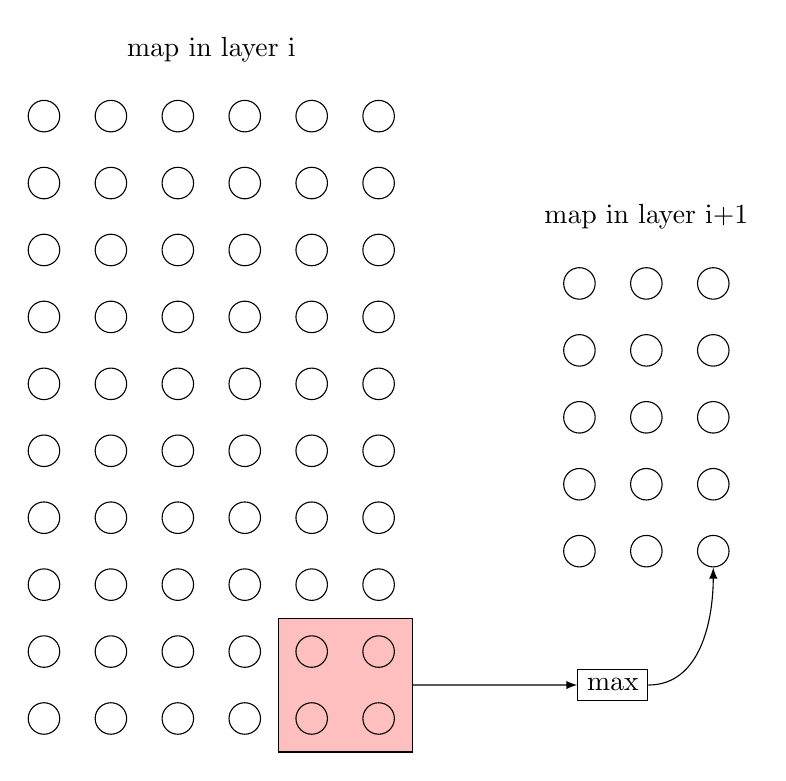
\begin{tikzpicture}[scale=0.85,every path/.style={>=latex}]
		\node (layeri) at (2.5,10) {map in layer i};
		\node (layeri) at (9,7.5) {map in layer i+1};
	
     	% draw background for max pooling
     	\draw[fill=pink] (3.5,-0.5) rectangle (5.5,1.5);
     	
     	% draw left layer
     	\foreach \x in {0,...,5}
     	{
     		\foreach \y in {0,...,9}
     		{
     			\node(1-\x-\y) at (\x,\y) [circle,draw,minimum size=0.4cm] {};
     		}
     	}
     	
     	% draw right layer
     	\foreach \x in {0,...,2}
     	{
     		\foreach \y in {0,...,4}
     		{
     			\node(2-\x-\y) at (\x + 8,\y + 2.5) [circle,draw,minimum size=0.4cm] {};
     		}
     	}
     	
     	% draw "+" rectangle
     	\node (max) at (8.5,0.5) [draw,rectangle] {max};
     	
     	% draw line from red rectangle to max
     	\draw[->] (5.5,0.5) to (max);
     	
     	% draw line from max to corresponding neuron in layer i+1
     	\draw[->,out=0,in=270] (max) to (2-2-0);
	\end{tikzpicture}
	\caption{Max Pooling layer}
	\label{fig:max_pooling}
\end{figure}
